% filepath: /home/giuseppe/pmts/notebooks/GL_exam_report.tex
\documentclass[a4paper,11pt]{article}
\usepackage{graphicx}
\usepackage{amsmath}
\usepackage{hyperref}
\usepackage{geometry}
\geometry{margin=1in}

\title{Predictive Models for Time Series: Report}
\author{Giuseppe Lombardi}
\date{\today}

\begin{document}

\maketitle

\section{Introduction}
This report documents the workflow and results of the \texttt{GL\_exam.ipynb} notebook,
which addresses a multivariate time series classification task using the PMTSA\_2025 dataset.
The analysis includes data loading, preprocessing, exploratory analysis, imputation, and the application of several machine learning models.

\section{Data Loading}
The dataset is loaded using \texttt{xarray} with a custom backend (\texttt{pyrregular}).
The main data array has the shape $(N, C, T)$, where $N$ is the number of time series samples, $C$ is the number of channels, and $T$ is the number of timestamps.
The data is stored initially as a sparse array for efficiency, and it is converted in a dense form to be used by the predictive models.

\section{Datas Description}

The dataset used in this project is derived from the 2019 PhysioNet/Computing in Cardiology Challenge..
It consists of multivariate clinical time series data collected from pediatric intensive care unit (PICU) patients.

Each sample corresponds to a single patient stay, represented as a multivariate time series.
The time series are sampled each hour but have several missing values.
Each sample contains measurements from $C=34$ clinical channels (vital signs, laboratory results, etc.) over a $T=334$ number of timestamps.
Static variables such as age and gender are also provided for each patient.
The dataset is split into training and test sets, where the number of samples in the training set is $N_{tr}=20334$,
and the number of samples in the test set is $N_{ts}=1998$.

The target is a binary label $0$ or $1$ indicating whether the patient developed sepsis during their stay.
The target labels are provided only for the training set.

\section{Data Analysis}
The dataset is highly imbalanced, with a significant proportion of samples labeled as $0$ (no sepsis).
More precisely, the training set contains $18546$ samples labeled as $0$ and $788$ samples labeled as $1$,
with a percentage of $8.8\%$ for the positive class.
The distribution of labels in the training set is shown in Figure \ref{fig:labels_tr}.
\begin{figure}[htbp]
\centering
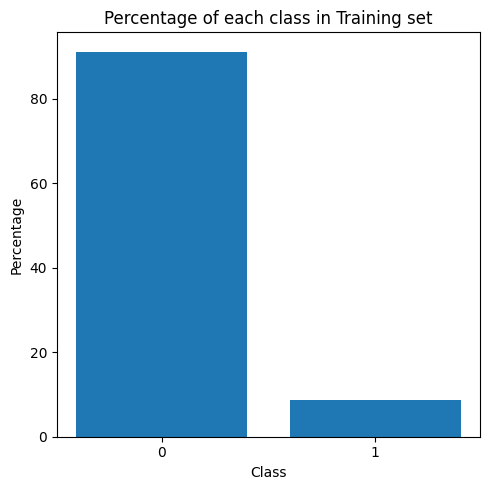
\includegraphics[width=0.5\textwidth]{imgs/labels_tr.png}
\caption{Distribution of labels in the training set.}
\label{fig:labels_tr}
\end{figure}

The main problem with the dataset is the presence of missing values, which are common in clinical data.
The dataset contains a significant amount of missing values, with an initial percentage of missing values around $97.6\%$ for the training set and $97.8\%$ for the test set.
In a first phase we analyse particularly the missing values in the training set to understand the distribution of missing values across samples, channels, and timestamps.

We plot for each sample ID in the training set the percentage of missing values across all channels and timestamps.
The distribution of missing values across samples is shown in Figure \ref{fig:missing_values_samples}.
\begin{figure}[htbp]
\centering
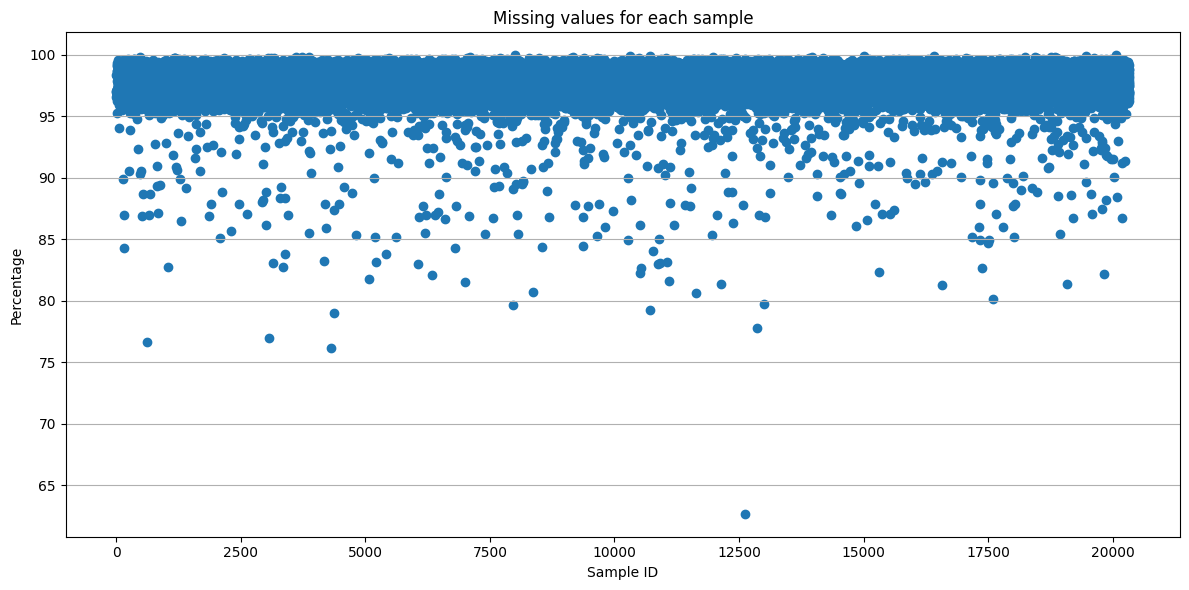
\includegraphics[width=1.0\textwidth]{imgs/missing_values_samples.png}
\caption{Distribution of missing values across samples in the training set.}
\label{fig:missing_values_samples}
\end{figure}

The dataset includes a variety of physiological and laboratory measurements, such as heart rate, blood pressure, respiratory rate, temperature, oxygen saturation, and several blood test results.
Not all channels are present for every patient and timestamp, resulting in channels that are not useful for the classification task.
To understand what are the most important channels for the classification task, we plot the distribution of missing values across the distinct channels.
All channels have a percentage of missing values greater than $89\%$, and only $5$ channels have a percentage of missing values lower than $91\%$.
\begin{figure}[htbp]
\centering
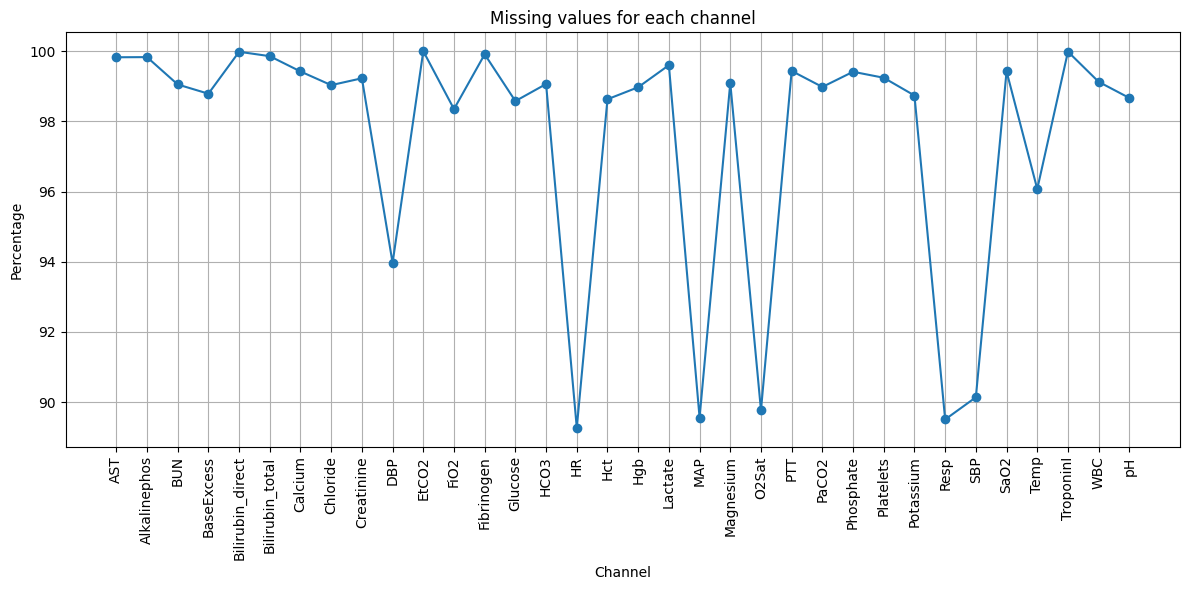
\includegraphics[width=1.0\textwidth]{imgs/missing_values_channels.png}
\caption{Distribution of missing values across channels in the training set.}
\label{fig:missing_values_channels}
\end{figure}
The distribution of missing values across channels is shown in Figure \ref{fig:missing_values_channels}.

\textbf{References:}
\begin{itemize}
    \item \href{https://www.kaggle.com/competitions/2025-predictive-models-for-time-series-analysis}{Kaggle Competition Page}
    \item \href{https://physionet.org/content/challenge-2019/1.0.0/}{PhysioNet Challenge 2019}
\end{itemize}

\section{Preprocessing}
\begin{itemize}
    \item \textbf{Channel Filtering:} Channels with more than 90\% missing values were removed.
    \item \textbf{Timestamp Cutoff:} Only the first 10 timestamps were retained.
    \item \textbf{Sample Filtering:} Samples with more than 20\% missing values were excluded.
    \item \textbf{Label Encoding:} Class labels were encoded using \texttt{LabelEncoder}.
    \item \textbf{Imputation:} 
        \begin{itemize}
            \item Fully missing channels were filled with the mean of the corresponding channel.
            \item Remaining missing values were imputed using the \texttt{drift} method from \texttt{sktime}'s \texttt{Imputer}.
        \end{itemize}
\end{itemize}

\section{Machine Learning Models}
Several models were trained and evaluated using cross-validation and grid search:
\begin{itemize}
    \item \textbf{Euclidean KNN:} \texttt{KNeighborsTimeSeriesClassifier} with Euclidean distance.
    \item \textbf{CNN:} Deep learning classifier (\texttt{CNNClassifier}) with hyperparameter tuning.
    \item \textbf{ROCKET:} Kernel-based classifier (\texttt{RocketClassifier}) with optional scaling.
    \item \textbf{Catch22 + RF:} Feature extraction (\texttt{Catch22}) followed by a Random Forest classifier.
    \item \textbf{Dummy Classifier:} Baseline for comparison.
\end{itemize}

\section{Results}
\begin{itemize}
    \item Best hyperparameters were selected for each model using \texttt{GridSearchCV} with F1 score as the metric.
    \item The performance of each model was evaluated on the test set.
    \item Submission files were generated for each model.
\end{itemize}

\section{Conclusion}
The notebook demonstrates a complete pipeline for multivariate time series classification, including advanced preprocessing and the application of state-of-the-art models. Further improvements could include more sophisticated imputation, feature engineering, or ensemble methods.

\section*{Appendix}
\begin{itemize}
    \item Code and plots are available in the accompanying Jupyter notebook.
    \item Libraries used: \texttt{xarray}, \texttt{numpy}, \texttt{matplotlib}, \texttt{sktime}, \texttt{scikit-learn}, \texttt{pandas}.
\end{itemize}

\end{document}